% =============================================================================
% Section 4: Architecture and Formal Semantics (RESTRUCTURED)
% =============================================================================

\subsection{Document Model: L1--L4 as Conceptual Modelling Layers}\label{subsec:document-model}

ADL Lite organises capability documents into four semantic layers, each with distinct syntax, role, and corresponding event types. The layering separates identity metadata (L1), narrative content (L2), typed assertions (L3), and executable actions (L4), enabling both human readability and machine processing within a single Markdown file. Table~\ref{tab:document-model} summarises the document model.

\begin{table}[htbp]
\centering
\small
\caption{The L1--L4 Document Model. Each layer contributes distinct semantics to the capability document.}
\label{tab:document-model}
\begin{tabular}{@{}p{1.2cm}p{3.2cm}p{4cm}p{4.5cm}@{}}
\toprule
\textbf{Layer} & \textbf{Syntax} & \textbf{Role} & \textbf{Event Type} \\
\midrule
L1 & YAML front matter & Identity metadata (derived snapshot) & SNAPSHOT \\
L2 & Markdown body & Human/LLM narrative prose & --- \\
L3 & \texttt{adl:relation}, \texttt{adl:evidence}, \texttt{adl:seal} & Typed semantic assertions & RELATE, EVIDENCE, SEAL \\
L4 & \texttt{adl:action} & Typed actions with preconditions & REGISTER, VALIDATE, DEPRECATE, \ldots \\
\bottomrule
\end{tabular}
\end{table}

The L1 layer comprises YAML front matter containing identity metadata; critically, these fields are \emph{derived snapshots} recomputed from the EventChain-record (the serialized information content entity, see \S\ref{subsec:two-level-account}). The L2 layer consists of Markdown body prose subject to the Singular Subjectivity Assertion (SSA).

\textbf{Definition (SSA).} The Singular Subjectivity Assertion is a document-level constraint stating that every L2 Markdown body is authored by a single actor at a single time. It is enforced by the parser: any L2 section containing multiple contradictory subjective claims without explicit attribution is flagged as an SSA violation. The SSA ensures that the L2 narrative layer remains traceable to a single source of subjectivity, preventing ``ghost-authored'' reasoning. Contradictory subjective assertions must be recorded as separate L4 events (e.g., \textsc{Evidence} or \textsc{Relate}) by different actors. The SSA interacts with lifecycle audit as follows: (i)~a concept in \texttt{provisional} status may contain SSA-violating prose (it is unvalidated); (ii)~a \textsc{Validate} action's precondition requires that the L2 body pass SSA checking; (iii)~\textsc{Fork} events inherit the parent's L2 body but must satisfy SSA for the new actor's rationale. Basic SHACL shapes are implemented (Appendix~\ref{app:implementation}); full SSA-specific SHACL enforcement and epistemic context learning remain future work (FW6).

The L3 layer introduces typed semantic assertions through fenced blocks supporting predicates such as \texttt{isomorphic-to}, \texttt{specialisation-of}, and \texttt{related-to}. If two agents independently register ``gradient-explosion'' and ``exploding-gradients'', the recommended workflow detects the near-duplicate through string similarity and links them with the strongest applicable predicate (\texttt{isomorphic-to} for structural equivalence). Automated canonicalisation via embedding clustering is deferred to future work (FW7).

\textbf{Invariant 2 (L3 Relation Reconciliation).} When either the source or target concept of a \texttt{RELATE} event undergoes a state transition to \texttt{deprecated} or \texttt{archived}, the relation's validity is determined by the status of both endpoint concepts. A relation is valid only if at least one endpoint is in \texttt{validated} status and neither endpoint is in \texttt{archived} or \texttt{deprecated} status. Let $r$ be a relation with predicate $p$ from concept $C_1$ to concept $C_2$, and let $S(C)$ denote the current lifecycle status of concept $C$. Then:
\begin{align}
    \text{valid}(r) \iff{}& S(C_1) \notin \{\text{archived}, \text{deprecated}\} \land S(C_2) \notin \{\text{archived}, \text{deprecated}\} \nonumber \\
    &{}\land \bigl(S(C_1) = \text{validated} \lor S(C_2) = \text{validated}\bigr).
\end{align}
Relations with at least one endpoint in \texttt{validated} status and no endpoint in \texttt{archived} or \texttt{deprecated} status remain valid for query and traversal. Conversely, relations between two \texttt{provisional} concepts, or where either endpoint is \texttt{deprecated} or \texttt{archived}, are excluded from the warm index. If a forked concept $C'$ is created via a \texttt{FORK} event from $C$, the parent concept retains all existing relations, whereas $C'$ inherits \texttt{isomorphic-to} and \texttt{specialisation-of} links from $C$. It does not inherit \texttt{analogical-to} links, which are re-evaluated during the forking agent's validation workflow. This invariant ensures that the relation graph remains navigable during multi-agent reorganisation and that stale or superseded edges do not pollute semantic queries.

\subsection{EventChain: Core Data Structure}\label{subsec:eventchain}

The EventChain-record (the serialized information content entity, see \S\ref{subsec:two-level-account}) is the fundamental data structure of ADL Lite: an append-only sequence of hash-linked events. An event comprises ten fields: \texttt{event\_id}, \texttt{concept\_id}, \texttt{event\_type}, \texttt{actor}, \texttt{reasoning}, \texttt{timestamp}, \texttt{payload}, \texttt{previous\_event\_id}, \texttt{hash}, and an optional \texttt{signature} (for Ed25519 signature verification, \S\ref{subsec:trust-model}). The event type system is partitioned into lifecycle events $\Sigma_{\text{life}}$ and communication events $\Sigma_{\text{comm}}$:

\begin{align}
    \Sigma_{\text{life}} &= \{\text{REGISTER},\; \text{VALIDATE},\; \text{DEPRECATE},\; \text{FORK},\; \text{ARCHIVE}\} \\
    \Sigma_{\text{comm}} &= \{\text{RELATE},\; \text{EVIDENCE},\; \text{SEAL},\; \text{ANNOUNCE},\; \text{PUBLISH},\; \text{SNAPSHOT}, \nonumber \\
    &\qquad\; \text{CALIBRATE},\; \text{SYNC\_DASHBOARD},\; \text{LISTEN},\; \text{REVOKE}\}
\end{align}

\subsection{Canonical Serialization and Cryptographic Integrity}\label{subsec:crypto}

Each event's hash is computed from canonical JSON serialization with lexicographically sorted keys, six-decimal rounding, and the timestamp. The canonicalization policy is version-locked: a schema version identifier (\texttt{canon-v1}) is included in the hash input, ensuring that future changes to rounding precision or key ordering do not retroactively invalidate existing hashes. Integrity verification $\text{VerifyIntegrity}(C)$ checks four conditions for a chain $C = [e_1, \ldots, e_n]$: (1)~genesis anchoring ($e_1.\text{previous\_event\_id} = \text{null}$), (2)~cryptographic linkage ($e_i.\text{prev\_hash} = e_{i-1}.\text{hash}$), (3)~hash correctness ($e_i.\text{hash} = \text{SHA-256}(\text{Canon}(e_i))$), and (4)~no dangling \texttt{previous\_event\_id} on the genesis event. When $\text{full}=\text{true}$, it additionally verifies archive file hashes against stored \texttt{archive\_pointer} values.\par
\textbf{Genesis hash stability and rehydration vulnerability.} The genesis hash is the hash of the first \textsc{Register} event, which includes the \texttt{concept\_id}; early versions excluded it, causing collisions when different concepts shared the same initial payload (corrected in E1, \S\ref{subsec:e1}). The canonical JSON serializer normalises line endings to LF and encodes Unicode as UTF-8; the version-locked \texttt{canon\_version} field pins the serialization policy so that benign formatting changes (e.g., prettier Markdown reformatting) do not affect event hashes. When a chain is copied across repositories, two failure modes can fragment identity: \emph{formatting drift} (different line endings or key ordering break the recomputed hash; mitigated by \texttt{canon\_version}) and \emph{metadata injection} (external systems adding fields such as a \texttt{signature} to legacy events change the canonical JSON). ADL Lite therefore treats the genesis hash as \emph{write-once}: any migration adding new fields must store them in subsequent events, not retroactively modify the genesis event. The formal resilience criterion is: a chain $C$ rehydrated in repository $R'$ satisfies $\text{VerifyIntegrity}(C) = \text{true}$ if and only if $C$ was well-formed in the source repository $R$ and no event content was modified during transfer.

\subsubsection{Dual-Identifier Design: Content Addressability}
\label{subsubsec:dual-identifier}

ADL Lite uses a \emph{dual-identifier} scheme separating \emph{provenance identity} (\emph{who} created the concept and \emph{when}) from \emph{content identity} (\emph{what} the concept semantically describes), addressing the identity-proliferation problem in multi-agent authoring.

\textbf{Genesis hash (provenance identity).} The genesis hash $h_{\text{gen}} = \text{SHA-256}(\text{Canon}(e_{\text{REG}}))$ includes the \texttt{concept\_id}, the actor's identifier, and the creation timestamp; it is \emph{unique per registration event} (two agents registering the same capability at different times yield different hashes) and is the \emph{primary identifier} for all lifecycle audit.

\textbf{Content hash (content identity).} The content hash $h_{\text{content}} = \text{SHA-256}(\text{Canon}(\text{L2\_body}, \text{L3\_blocks}))$ excludes all registration-varying metadata; it is \emph{stable across independent registrations} with identical (or near-identical, within a configurable Levenshtein threshold) L2/L3 descriptions.

\textbf{Near-duplicate detection.} On \textsc{Register}, if $h_{\text{content}}$ matches an existing concept (exact or within a Levenshtein ratio threshold of 0.85), the ActionExecutor emits an advisory warning (``This concept may be a duplicate of [existing concept]...'') suggesting a \textsc{Relate} event with predicate \texttt{isomorphic-to}; the agent may still register a separate entity. The content hash is computed in $O(|\text{L2}| + |\text{L3}|)$ time, is stored in the event payload, and is \emph{not} part of the cryptographic chain (it is an advisory field, so it does not affect well-formedness or integrity).

\textbf{Formal resilience criteria and DID vs.~content-linked PID comparison.} Any identity mechanism must satisfy: (i)~\emph{provenance uniqueness} (distinct identifiers for identical content), (ii)~\emph{rehydration stability} (identifier preserved across repository copies unless content changes), and (iii)~\emph{content-addressability option} (secondary content-derived identifier for near-duplicate detection). $h_{\text{gen}}$ satisfies (i)--(ii); $h_{\text{content}}$ satisfies (iii). A content-addressed PID (IPFS CID) would satisfy (ii)--(iii) but fail (i) by colliding on identical content; a DID (\texttt{did:key}) satisfies (i) but fails (ii) because DIDs are not content-sensitive. The dual-identifier scheme is the minimal design satisfying all three criteria simultaneously; Table~\ref{tab:identity-comparison} summarises the comparison.

\begin{table}[htbp]
\centering
\small
\caption{Identity mechanism comparison: genesis hash, content hash, DID, and content-addressed PID.}
\label{tab:identity-comparison}
\begin{tabularx}{\textwidth}{@{}p{2.5cm}p{2.5cm}p{2.5cm}p{2.5cm}X@{}}
\toprule
\textbf{Criterion} & \textbf{$h_{\text{gen}}$} & \textbf{$h_{\text{content}}$} & \textbf{DID} & \textbf{Content PID} \\
\midrule
Provenance uniqueness & $\checkmark$ & $\times$ & $\checkmark$ & $\times$ \\
Rehydration stability & $\checkmark$ & $\checkmark$ & $\times$ & $\checkmark$ \\
Content-addressability & $\times$ & $\checkmark$ & $\times$ & $\checkmark$ \\
Cryptographic binding & $\checkmark$ & $\times$ & $\checkmark$ & $\checkmark$ \\
Human readability & $\times$ & $\times$ & $\checkmark$ & $\times$ \\
\bottomrule
\end{tabularx}
\end{table}

\subsection{Precondition Language and Action Executor}\label{subsec:precondition-executor}

\subsubsection{Formal Precondition Language}\label{subsubsec:precondition-language}

L4 action blocks are validated against preconditions expressed in a constrained, decidable language. A precondition rule is a triple $\langle \text{field}, \text{comparator}, \text{value} \rangle$ with comparator alphabet $\mathcal{K} = \{\text{EQ}, \text{NEQ}, \text{GT}, \text{GTE}, \text{LT}, \text{LTE}, \text{IN}, \text{EXISTS}\}$. Table~\ref{tab:comparator-semantics} gives the formal semantics.

\begin{table}[htbp]
\centering
\small
\caption{Comparator semantics: explicit operator mapping to ground predicates.}
\label{tab:comparator-semantics}
\begin{tabular}{@{}p{2.5cm}p{3cm}p{5.5cm}@{}}
\toprule
\textbf{Comparator} & \textbf{Predicate} & \textbf{FOL encoding} \\
\midrule
EQ & Equality & $x = y$ \\
NEQ & Disequality & $\neg(x = y)$ \\
GT & Greater than & $x > y$ \\
GTE & Greater than or equal & $x \geq y$ \\
LT & Less than & $x < y$ \\
LTE & Less than or equal & $x \leq y$ \\
IN & Set membership & $x \in Y$ (where $Y$ is a finite set) \\
EXISTS & Non-null check & $\exists x \,:\, x \neq \text{null}$ \\
\bottomrule
\end{tabular}
\end{table}

\textbf{BNF grammar.} Let $\mathcal{N}$ be the set of alphanumeric field identifiers, $\mathcal{S} = \mathbb{R} \cup \mathbb{B} \cup \Sigma^*$ the set of scalar literals (reals, booleans, strings), and $\mathcal{P}_{\text{fin}}(\mathcal{S})$ the finite power set of scalars. The precondition language $\mathcal{L}_{\text{pre}}$ is generated by the grammar $G = (\mathcal{V}, \Sigma_{\text{term}}, R, \text{rule\_list})$ with non-terminals $\mathcal{V} = \{\text{rule\_list}, \text{rule}, \text{field}, \text{comparator}, \text{value}\}$, terminals $\Sigma_{\text{term}} = \mathcal{N} \cup \mathcal{S} \cup \{\text{EQ}, \text{NEQ}, \text{GT}, \text{GTE}, \text{LT}, \text{LTE}, \text{IN}, \text{EXISTS}, \text{AND}, \text{OR}, \text{null}\}$, and production rules $R$:
{\small
\begin{align*}
    \text{rule\_list} &::= \text{rule} \;\mid\; \text{rule\_list} \; \text{AND} \; \text{rule\_list} \;\mid\; \text{rule\_list} \; \text{OR} \; \text{rule\_list} \\
    \text{rule} &::= \langle \text{field}, \text{comparator}, \text{value} \rangle \\
    \text{field} &::= f \in \mathcal{F} \quad (\text{the finite set of snapshot field names}) \\
    \text{comparator} &::= \text{EQ} \mid \text{NEQ} \mid \text{GT} \mid \text{GTE} \mid \text{LT} \mid \text{LTE} \mid \text{IN} \mid \text{EXISTS} \\
    \text{value} &::= s \in \mathcal{S} \mid P \in \mathcal{P}_{\text{fin}}(\mathcal{S}) \mid \text{null}
\end{align*}
}

\textbf{Formal semantics.} Let $\mathcal{D}$ be the domain of values (scalars, sets, and $\text{null}$). Let $\text{Snapshot}(C)$ be the derived snapshot of chain $C$, a finite map from field names to $\mathcal{D}$. The semantic function $\text{eval}(r, C) \in \{\text{true}, \text{false}\}$ is defined for a rule $r = \langle f, \kappa, v \rangle$ by:
\begin{equation}
    \text{eval}(\langle f, \kappa, v \rangle, C) = \text{apply}(\kappa, \text{lookup}(f, C), v)
\end{equation}
where $\text{lookup}(f, C) = \text{Snapshot}(C)[f]$ (the value of field $f$ in the snapshot, or $\text{null}$ if absent), and $\text{apply}(\kappa, x, y)$ is the comparator-specific predicate from Table~\ref{tab:comparator-semantics}. The snapshot is pre-computed in $\mathcal{O}(n)$ time by a single scan of $C$; subsequent rule evaluations are $\mathcal{O}(1)$.

\textbf{Composition semantics.} A rule list $R = [r_1, \ldots, r_k]$ is evaluated as a conjunction: $\text{eval}(R, C) = \bigwedge_{i=1}^{k} \text{eval}(r_i, C)$. Evaluation is short-circuit: if $\text{eval}(r_j, C) = \text{false}$ for any $j < k$, the remaining rules are not evaluated. The language is a variable-free ground fragment: each rule is a single atomic comparison over a cached derived snapshot, with no quantification, no recursion, and no dynamic code execution. The conjunction of $k$ rules is a variable-free conjunction of ground atoms, evaluated in $\mathcal{O}(k)$ time (Theorem~8).

Precondition evaluation is pure and referentially transparent: it references only the snapshot of the chain $C$ being validated, and does not access external chains, databases, or network resources. Cross-chain preconditions (e.g., ``allow \textsc{Validate} only if concept $X$ is \texttt{validated}'') are not supported in the core language; they are deferred to future work (FW2). This local-scope restriction ensures that precondition evaluation is deterministic and executable without consensus or network access.

\paragraph{Static typing.} A rule $\langle f, \kappa, v \rangle$ is well-typed, denoted $\vdash \langle f, \kappa, v \rangle : \text{bool}$, iff $\text{type}(f) \in \mathcal{T} = \{\mathbb{R}, \mathbb{B}, \Sigma^*, \mathcal{P}_{\text{fin}}(\mathcal{S})\}$ and the comparator--value pair satisfies the compatibility predicate: $\text{EQ}/\text{NEQ}$ require $\text{type}(f) = \text{type}(v)$ with $v \in \mathcal{S}$; $\text{GT}/\text{GTE}/\text{LT}/\text{LTE}$ require $\text{type}(f) = \mathbb{R}$ and $v \in \mathbb{R}$; $\text{IN}$ requires $v \in \mathcal{P}_{\text{fin}}(\mathcal{S})$ with $\text{type}(f) = \text{type}(v_i)$ for all $v_i \in v$; $\text{EXISTS}$ requires $\text{type}(f) \in \mathcal{T}$ with $v = \text{null}$. The ActionExecutor rejects any rule violating $\vdash$ before evaluation, so $\llbracket \rho \rrbracket(\sigma)$ never encounters a runtime type error. The evaluation function is defined by exhaustive case analysis on the comparator---e.g., $\text{eval}(\sigma, \langle f, \text{EQ}, v \rangle) = (\sigma.f = v)$, $\text{eval}(\sigma, \langle f, \text{GT}, v \rangle) = (\sigma.f > v)$, $\text{eval}(\sigma, \langle f, \text{IN}, vs \rangle) = (\sigma.f \in vs)$, $\text{eval}(\sigma, \langle f, \text{EXISTS}, \text{null} \rangle) = (\sigma.f \neq \text{null})$; the remaining comparators (NEQ, GTE, LT, LTE) follow analogously.

\paragraph{Safety.} The precondition language contains no \texttt{eval()}, no \texttt{exec()}, and no dynamic code execution. Comparator dispatch is a closed enumeration: the Python implementation uses a fixed \texttt{Comparator} enum with eight explicit cases, so no user-supplied string can be interpreted as code. Because $\sigma$ is a precomputed hash map, field lookup is $O(1)$; because the comparator cases are a closed enumeration of primitive operations, each comparison is $O(1)$.

\subsubsection{Complexity Analysis}\label{subsubsec:complexity-analysis}

\paragraph{Theorem (Precondition Evaluation Complexity).} For any well-formed EventChain $C$ with cached snapshot $\sigma$ and any list of $k$ precondition rules $R = [r_1, \ldots, r_k]$, total evaluation time is $O(k)$, with $O(1)$ per rule and $O(1)$ auxiliary space.

\emph{Proof Sketch.} Each rule performs a single field lookup in $\sigma$ (a hash map, $O(1)$) and a closed comparison (a primitive operation, $O(1)$); the rule list is evaluated as a short-circuit conjunction with no quantification, recursion, or backtracking. The snapshot $\sigma$ is precomputed in $O(n)$ at append time, so the per-rule cost is $O(1)$ amortized. (Full proof in Appendix~\ref{app:proofs}.)

\paragraph{Empirical validation.} Experiment E34 (Precondition Formalization Benchmark) empirically confirms the $O(1)$ per-rule claim: per-rule evaluation measures $0.8$--$1.0\,\mu\text{s}$, independent of chain length (tested up to $1{,}000$ events). This validates that the closed comparator dispatch and hash-map field lookup dominate the cost, with no superlinear term emerging from large snapshots.

\subsubsection{Precondition Language Expressivity}

The precondition language is intentionally minimal: a variable-free ground fragment with eight comparators, no recursion, no quantification, and no dynamic code execution. This minimalism guarantees decidability and $\mathcal{O}(1)$ per-rule evaluation (Theorem~8), at the cost of expressivity (Supplementary Table S12 classifies the boundaries). Time is not a first-class value: temporal constraints are enforced at the application layer, and cross-chain predicates are unsupported by design (the language evaluates only the snapshot of the chain being modified, ensuring referential transparency and eliminating the need for distributed consensus; cross-chain references would introduce non-determinism).

\textbf{Theorem~8 (Precondition Evaluation Termination and Complexity).} For any well-formed EventChain $C$ and any precondition rule $r$, $\text{eval}(r, C)$ terminates in $\mathcal{O}(1)$ time (assuming the derived snapshot is cached). For a list of $k$ rules, total time is $\mathcal{O}(k)$ and space is $\mathcal{O}(1)$. \emph{Proof Sketch:} Both field lookup and comparator dispatch are $\mathcal{O}(1)$; the language contains no recursion or quantification. See Appendix~\ref{app:proofs} for the full decidability proof. Supplementary Table S13 summarises the complexity; the decidability and complexity-class discussion (membership in \textbf{P}) is in Appendix~H.

\textbf{Complete lifecycle transition matrix.} Table~\ref{tab:lifecycle-matrix} lists the ActionExecutor preconditions for each lifecycle event (encoded in \texttt{adl\_core\_ontology.yaml}). Under CRDT LUB semantics, the final status is the maximum over all lifecycle events, not the last event; the ActionExecutor still enforces preconditions to prevent semantically nonsensical sequences (e.g., archiving a concept never validated).

\begin{table}[htbp]
\centering
\footnotesize
\caption{Lifecycle event preconditions: permitted events from current status (rows). The final status is the LUB of all lifecycle events in the chain (CRDT semantics).}
\label{tab:lifecycle-matrix}
\begin{tabular}{@{}p{2cm}ccccc@{}}
\toprule
\textbf{Status} & \textsc{Reg.} & \textsc{Val.} & \textsc{Dep.} & \textsc{Fork} & \textsc{Arch.} \\
\midrule
provisional & $\times$ (gen.) & $\checkmark$ & $\checkmark$ & $\checkmark$ & $\checkmark$ \\
validated & $\times$ & $\checkmark$ (re) & $\checkmark$ & $\checkmark$ & $\checkmark$ \\
deprecated & $\times$ & $\checkmark$ & $\times$ & $\times$ & $\checkmark$ \\
forked & $\times$ & $\checkmark$ & $\checkmark$ & $\times$ & $\checkmark$ \\
archived & $\times$ & $\times$ & $\times$ & $\times$ & $\times$ \\
\bottomrule
\end{tabular}
\end{table}

\textsc{Register} is permitted only as a genesis event (creating a new concept). From \texttt{validated}, \textsc{Validate} is permitted as a re-validation (adding a new confidence assertion). Under CRDT LUB semantics, once a chain reaches \texttt{deprecated}, subsequent \textsc{Validate} events do not change the status back to \texttt{validated} (the LUB of \texttt{deprecated} and \texttt{validated} is \texttt{deprecated}), but they can still be appended as auditable evidence. Re-activation after deprecation requires a new \textsc{Register} event (new genesis), not a reversal of the existing chain.

\subsubsection{Action Executor and Transition Engine}\label{subsubsec:action-consensus}

The ActionExecutor validates L4 action blocks against a closed action registry defined in \path{adl\_core\_ontology.yaml}. Each action definition specifies preconditions as a list of \texttt{PreconditionRule} objects. The ConsensusEngine governs the resulting status transitions by appending events to the chain; the final status is derived via the CRDT LUB over all lifecycle events (Theorem~1), not by a transition matrix. Forking creates a new child chain with a fresh \texttt{REGISTER} event while the original chain's status is the LUB of its previous status and \texttt{forked}; both evolve independently.

\subsection{Compact Formal Specification}\label{subsec:compact-formal-spec}

This subsection presents a \emph{single-page, self-contained} formal specification of ADL Lite's derivation semantics. All definitions, theorems, and complexity claims are stated here; expanded proof sketches and sensitivity analysis appear in Appendix~E. The specification is organised as: (i)~the status lattice and derivation function~$\delta$; (ii)~the confidence aggregation function~$\gamma$ (three variants); (iii)~the precondition language; and (iv)~the fork and merge semantics.

\subsubsection{Status Lattice and Derivation Function $\delta$}\label{subsubsec:status-lattice}

Let $\Sigma = \Sigma_{\text{life}} \cup \Sigma_{\text{comm}}$ be the event alphabet. The lifecycle events are $\Sigma_{\text{life}} = \{\text{REGISTER},\; \text{VALIDATE},\; \text{DEPRECATE},\; \text{FORK},\; \text{ARCHIVE}\}$. The communication events are $\Sigma_{\text{comm}} = \{\text{RELATE},\; \text{EVIDENCE},\; \text{SEAL},\; \text{ANNOUNCE},\; \text{PUBLISH},\; \text{SNAPSHOT},\; \text{CALIBRATE},\; \text{SYNC\_DASHBOARD},\; \text{LISTEN},\; \text{REVOKE}\}$. A chain $C = [e_1, \ldots, e_n]$ is well-formed, denoted $\text{WF}(C)$, if it satisfies 13 axioms: genesis anchoring, shared \texttt{concept\_id}, cryptographic linkage, hash correctness, distinct \texttt{event\_id}, non-empty actor, timestamp monotonicity, payload schema conformance, action preconditions, scope ACL, signature verification, confidence clamping, and valid event type (the full list is in Appendix~E).

The status space is $S = \{\text{provisional},\; \text{forked},\; \text{validated},\; \text{deprecated},\; \text{archived}\}$, equipped with the total order:
\begin{equation}\label{eq:status-order}
    \text{provisional} \;\prec\; \text{forked} \;\prec\; \text{validated} \;\prec\; \text{deprecated} \;\prec\; \text{archived}
\end{equation}
numbered $1, 2, 3, 4, 5$ respectively. This is a join-semilattice: the least upper bound (LUB) of any subset is its maximum element. The status map $f: \Sigma_{\text{life}} \to S$ assigns $f(\text{REGISTER}) = \text{provisional}$, $f(\text{VALIDATE}) = \text{validated}$, $f(\text{DEPRECATE}) = \text{deprecated}$, $f(\text{FORK}) = \text{forked}$, $f(\text{ARCHIVE}) = \text{archived}$.

Let $C_{\text{life}} = \{e \in C \mid e.\tau \in \Sigma_{\text{life}}\}$ be the lifecycle subsequence. The status derivation function $\delta: \{C \mid \text{WF}(C)\} \to S$ is:
\begin{equation}\label{eq:delta-def}
    \delta(C) = \begin{cases}
        \text{provisional} & \text{if } C_{\text{life}} = \emptyset \\
        \max_{\prec}\{ f(e.\tau) \mid e \in C_{\text{life}} \} & \text{otherwise}
    \end{cases}
\end{equation}
where $\max_{\prec}$ is the maximum over the integer order (Eq.~\ref{eq:status-order}). Complexity: $O(|C|)$ by single scan of $C$ (or $O(1)$ with an incremental LUB cache updated on every \texttt{append}).

Under Eq.~\ref{eq:delta-def}, status is determined by the \emph{highest} lifecycle event in the lattice, not the last. Once $\text{deprecated}$ or $\text{archived}$ appears, no subsequent event can lower the status (monotonicity). Re-activation after deprecation requires a new genesis event on a new chain.

\subsubsection{Formal Lattice Structure}\label{subsubsec:formal-lattice}

The status space $S = \{\text{provisional}, \text{forked}, \text{validated}, \text{deprecated}, \text{archived}\}$ equipped with the total order $\prec$ (Eq.~\ref{eq:status-order}) forms a complete lattice $(S, \preceq, \sqcap, \sqcup, \bot, \top)$ where:
\begin{itemize}
    \item $\bot = \text{provisional}$ is the least element,
    \item $\top = \text{archived}$ is the greatest element,
    \item the join operator $\sqcup: S \times S \to S$ is defined by $\sqcup = \text{status\_max} = \max_{\prec}$, the least upper bound under $\prec$,
    \item the meet operator $\sqcap: S \times S \to S$ is defined by $\sqcap = \text{status\_min} = \min_{\prec}$, the greatest lower bound under $\prec$.
\end{itemize}
Because $\prec$ is a total order on a finite set, every subset $X \subseteq S$ (finite or infinite, though $S$ itself is finite) has both a maximum element $\max_{\prec} X$ and a minimum element $\min_{\prec} X$. Therefore every subset has a least upper bound and a greatest lower bound, and $(S, \preceq, \sqcap, \sqcup, \bot, \top)$ is a complete lattice~\cite{davey_priestley_2002}. The completeness is essential for CRDT convergence: the merge of any set of concurrent branches computes $\bigsqcup X$ for the lifecycle events $X$ of the merged chain, which is guaranteed to exist and be unique (Theorem~9).

\begin{figure}[htbp]
\centering
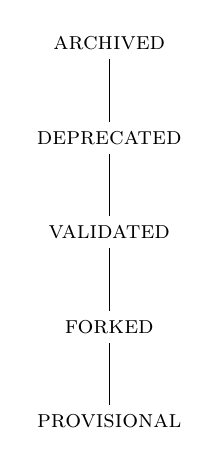
\begin{tikzpicture}[scale=1.2, every node/.style={font=\small}]
    \node (arch) at (0,4) {\textsc{archived}};
    \node (dep)  at (0,3) {\textsc{deprecated}};
    \node (val)  at (0,2) {\textsc{validated}};
    \node (fork) at (0,1) {\textsc{forked}};
    \node (prov) at (0,0) {\textsc{provisional}};
    \draw (prov) -- (fork);
    \draw (fork) -- (val);
    \draw (val) -- (dep);
    \draw (dep) -- (arch);
\end{tikzpicture}
\caption{Hasse diagram of the status lattice $(S, \preceq, \sqcup, \bot, \top)$. The diagram is a linear chain because $\prec$ is a total order.}
\label{fig:status-hasse}
\end{figure}

\paragraph{Join-semilattice proof.} Because $\prec$ is a total order on a finite set, $\sqcup = \max_{\prec}$ is associative, commutative, idempotent, has identity $\bot=\text{provisional}$, and is monotone (if $a \preceq b$ then $a \sqcup c \preceq b \sqcup c$). These properties are machine-verified in Coq (\texttt{Status.v}, Theorem~T3) and hold for the CRDT merge semantics (Theorem~T9); the identity property justifies the $O(1)$ incremental LUB cache (appending a non-lifecycle event, which contributes $\bot$, leaves the status unchanged). The meet operator $\sqcap = \min_{\prec}$ satisfies the dual five properties and is required only for the complete-lattice structure and future query semantics; the full algebraic enumeration is in Appendix~\ref{app:proofs}.

\subsubsection{Confidence Aggregation: Three Variants}

Let $V = [e \in C \mid e.\tau = \text{VALIDATE}]$ denote the validation subsequence. ADL Lite provides three confidence aggregation strategies.

\textbf{Variant 1: Default (G-Counter max).} The simplest strategy, used by default, takes the maximum confidence across all \texttt{VALIDATE} events (or \texttt{SNAPSHOT} if no validation has occurred):
\begin{equation}\label{eq:gamma-default}
    \gamma_{\text{default}}(C) = \begin{cases}
        0.0 & \text{if } V = [] \\
        \text{clamp}_{[0,1]}\bigl(\max\{ e.\text{payload}[\text{``confidence''}] \mid e \in V \}\bigr) & \text{otherwise}
    \end{cases}
\end{equation}
where $\max$ is over all validation events (G-Counter semantics) and $\text{clamp}_{[0,1]}(x) = \max(0, \min(1, x))$. It is evaluated in $O(1)$ time by an incremental cache (\texttt{\_cached\_confidence}) that updates to $\max(\text{cache}, \text{clamp}(c))$ on every append; the canonical state is always recomputable from the event sequence in $O(|V|) \leq O(n)$, so the $O(1)$ claim refers to the memoized warm-index query, not the canonical derivation.

\textbf{Variant 2: Bonus-formula aggregate ($\gamma_{\text{agg}}$).} Mitigates collusion by aggregating per-actor maxima and adding a bonus for cross-validation:
\begin{equation}\label{eq:gamma-agg}
    \gamma_{\text{agg}}(C) = \begin{cases}
        0.0 & \text{if } V = [] \\
        \min\!\bigl(1.0,\; c_{\text{base}} + 0.05 \times (N_{\text{vals}} - 1)\bigr) & \text{otherwise}
    \end{cases}
\end{equation}
where $N_{\text{vals}} = |\text{actors}(V)|$ and $c_{\text{base}} = \max(0.5, \frac{1}{N_{\text{vals}}} \sum_{a \in \text{actors}(V)} \phi(a, V))$, with $\phi(a, V) = \max\{e.\text{payload}[\text{``confidence''}] \mid e \in V \land e.\text{actor} = a\}$. The $0.05$ bonus per distinct validator rewards cross-validation; the $0.5$ floor prevents a single low-confidence validator from dominating (sensitivity analysis in Appendix~E).

\textbf{Variant 3: Calibrated confidence ($\gamma_{\text{cal}}$).} Weights each validator's confidence by a per-actor accuracy score:
\begin{equation}\label{eq:gamma-cal}
    \gamma_{\text{cal}}(C) = \begin{cases}
        0.0 & \text{if } V = [] \\
        \text{clamp}_{[0,1]}\!\Bigl(\frac{\sum_{a \in \text{actors}(V)} \text{accuracy}_a \cdot \phi(a, V)}{\sum_{a \in \text{actors}(V)} \text{accuracy}_a}\Bigr) & \text{otherwise}
    \end{cases}
\end{equation}
where $\text{accuracy}_a \in [0,1]$ is a per-actor accuracy score from an external calibration profile; complexity is $O(|V|)$.

\textbf{Concurrent resolution, bounds, and algebraic structure.} Concurrent lifecycle events commute because the LUB is order-independent (Eq.~\ref{eq:delta-def}); for $\gamma$, per-actor maxima are computed first, and concurrent events from the same actor commute because $\max$ is idempotent, so once a high-confidence validation is recorded, subsequent lower-confidence assertions cannot decrease the aggregate (Theorem~T5). All three variants are bounded in $[0,1]$ by construction: $\gamma_{\text{default}}$ uses $\text{clamp}_{[0,1]}$; $\gamma_{\text{agg}}$ uses $\min(1.0, \cdot)$ with $c_{\text{base}} \geq 0.5$; $\gamma_{\text{cal}}$ is a clamped convex combination (Theorem~T4, proved in Coq). Supplementary Table S30 summarises the algebraic structure: $\gamma_{\text{default}}$ is a pure G-Counter (max-semilattice) with full associativity, commutativity, and idempotence; $\gamma_{\text{agg}}$ and $\gamma_{\text{cal}}$ are commutative over the set of actors but not associative with respect to the full chain history, because their bonus/denominator terms depend on the cumulative actor set, which is not reconstructible from scalar intermediates. The incremental confidence cache satisfies $\text{cache} = \gamma(C)$ at all times (updated to $\max(\text{cache}, c)$ on \textsc{Validate} for $\gamma_{\text{default}}$; recomputed in $O(|V|)$ for $\gamma_{\text{agg}}$/$\gamma_{\text{cal}}$) and can be reconstructed by a single linear scan, so it is a pure optimisation, not a source of truth.

\textbf{Phase~1 limitations.} The current collaborative-audit model lacks authenticated identity, so $\gamma_{\text{cal}}$ accuracy scores are self-reported and do not prevent collusion (a single actor can report $\text{accuracy}_a = 1.0$); Sybil attacks are possible (one actor with $10$ pseudonyms can drive $\gamma_{\text{agg}}$ to $0.99$). These are known limitations (L3, \S\ref{subsec:limitations}), demonstrated in adversarial experiment E14 (Table~\ref{tab:undetectable-attacks}); mitigation requires authenticated identities and staking (Phase~3, FW9).

\subsubsection{Confidence as G-Counter CRDT}\label{subsubsec:confidence-gcounter}

The confidence function $\gamma_{\text{default}}(C)$ is a state-based G-Counter CRDT. Let $C$ be a chain and $V \subseteq C$ the subsequence of \textsc{Validate} and \textsc{Snapshot} events. The confidence is defined as:
\begin{equation}\label{eq:confidence-gcounter}
    \gamma(C) = \max\bigl(\{c \mid \exists e \in V : e.\text{payload}[\text{``confidence''}] = c\} \cup \{0\}\bigr)
\end{equation}

\paragraph{State-based G-Counter formalisation.} In the state-based CRDT model, the confidence G-Counter is the tuple $(\Sigma, \text{inc}, \text{merge}, s_0)$ where $\Sigma = [0,1]$ is the state type, $s_0 = 0$ the initial state, $\text{inc}(s, c) = \max(s, c)$ the increment, and $\text{merge}(s_1, s_2) = \max(s_1, s_2)$ the merge.

\begin{theorem}[Confidence is a State-Based G-Counter CRDT]\label{thm:confidence-gcounter}
The tuple $(\Sigma, \text{inc}, \text{merge}, s_0)$ defined above is a state-based G-Counter CRDT: the merge operation is associative, commutative, and idempotent, and the increment operation is monotonic with respect to the merge.
\end{theorem}
\emph{Proof Sketch.} $\text{merge} = \max$ is associative, commutative, and idempotent; $\text{inc}(s, c) = \max(s, c)$ is monotone in $s$; and confidence values are clamped to $[0,1]$, so the state never decreases. The full algebraic proof is in Appendix~\ref{app:proofs}.

The G-Counter semantics guarantee that once a high-confidence validation is recorded, subsequent lower-confidence assertions cannot decrease the aggregate (Theorem~T5). This monotonicity is critical for audit: validators cannot retrospectively weaken a concept's confidence by appending low-confidence events.

\subsubsection{Fork and Merge Semantics}\label{subsubsec:fork-merge}

A fork $\text{Fork}(C, a)$ appends a $\textsc{Fork}$ event to the parent chain and creates a child chain $C'$ with a fresh $\textsc{Register}$ event. The parent and child evolve independently:
\begin{align}
    \delta(C_{\text{fork}}) &= \max(\delta(C), \text{forked}) \quad \text{(parent status, LUB)} \\
    \delta(C') &= \text{provisional} \quad \text{(child status, fresh genesis)}
\end{align}
where $C_{\text{fork}} = C \oplus [e_{\text{FORK}}]$.

\textbf{Identity preservation under fork.} Let $C$ be a well-formed chain with genesis event $e_0$ and concept identifier $\textit{concept\_id}(C)$. The fork operation $\text{Fork}(C, a)$ produces $(C_{\text{fork}}, C')$ satisfying: (I1)~parent identity preservation, $\textit{concept\_id}(C_{\text{fork}}) = \textit{concept\_id}(C)$ and $h_{\text{gen}}(C_{\text{fork}}) = h_{\text{gen}}(C)$; (I2)~child identity distinctness, $h_{\text{gen}}(C') \neq h_{\text{gen}}(C)$ (fresh genesis with distinct timestamp and actor); and (I3)~lineage traceability, a $\textsc{Fork}$ event $e_{\text{FORK}} \in C_{\text{fork}}$ with $e_{\text{FORK}}.\text{payload}[\text{``child\_concept\_id''}] = \textit{concept\_id}(C')$ establishes a cryptographic link from parent to child. Conditions (I2)--(I3) ensure the parent and child are distinct concepts and that the lineage is auditable via the parent's EventChain.

\paragraph{LWW-Set merge formal definition.} Given concurrent well-formed branches $B_1, B_2$ derived from the same genesis event, the merged chain is defined as:
\begin{equation}\label{eq:lww-merge}
    \text{Merge}(B_1, B_2) = \text{Linearize}\bigl(\,\text{Dedup}(B_1 \cup B_2)\,\bigr)
\end{equation}
where $\text{Dedup}(E) = \{ e \in E \mid \nexists e' \in E : e' \neq e \land e'.\text{event\_id} = e.\text{event\_id} \}$ removes duplicate events by \texttt{event\_id}, and $\text{Linearize}(E)$ sorts the deduplicated set by the total order $\prec$ (Eq.~\ref{eq:total-order}). The merge satisfies the LWW-Set (Last-Write-Wins Set) semantics because the deduplication by \texttt{event\_id} ensures that the most recent (or only) version of each event is retained.

\textbf{Identity of the merge result.} Let $B_1, B_2$ be well-formed concurrent branches with shared genesis $e_0$ and common concept identifier $c$. The merged chain $M = \text{Merge}(B_1, B_2)$ satisfies: (M1)~$\textit{concept\_id}(M) = c$; (M2)~$h_{\text{gen}}(M) = h_{\text{gen}}(e_0) = h_{\text{gen}}(B_1) = h_{\text{gen}}(B_2)$; (M3)~every event from both branches appears exactly once in $M$ with all immutable content (\texttt{event\_id}, payload, actor, timestamp) preserved; and (M4)~optionally, the original branch hashes can be stored as metadata in a $\textsc{MERGE}$ event payload to provide ancestry proofs.

\paragraph{Re-anchor operation.} After linearization, the hash chain must be recomputed to restore cryptographic linkage. Let $E^* = [e^*_1, \dots, e^*_n]$ be the linearized merged event sequence. The re-anchor operation $\text{Reanchor}(E^*)$ computes:
\begin{align}
    e^*_1.\text{previous\_event\_id} &\gets \text{null}, \quad e^*_1.\text{prev\_hash} \gets \text{genesis}, \\
    \forall i > 1: \quad e^*_i.\text{previous\_event\_id} &\gets e^*_{i-1}.\text{event\_id}, \quad e^*_i.\text{prev\_hash} \gets \text{SHA-256}(\text{Canon}(e^*_{i-1})).
\end{align}
Each event's immutable content is preserved; only the linkage pointers are updated, so the merged chain has a \emph{different} hash sequence from either parent branch but all original event content is preserved (post-merge integrity, not pre-merge ancestry preservation).

\textbf{Total order $\prec$.} For events $e_i, e_j$:
\begin{equation}\label{eq:total-order}
    e_i \prec e_j \iff e_i.\text{timestamp} < e_j.\text{timestamp} \;\lor\; (e_i.\text{timestamp} = e_j.\text{timestamp} \;\land\; e_i.\text{event\_id} <_{\text{lex}} e_j.\text{event\_id})
\end{equation}
where $<_{\text{lex}}$ is lexicographic comparison of UUID strings. The order $\prec$ is a strict total order (reflexive closure $\preceq$, antisymmetry, transitivity, and totality all hold: timestamps are real numbers and UUID strings are totally ordered). Within a single chain, events are totally ordered by cryptographic linkage; across chains, the merge operation linearizes the merged set by sorting on $\prec$.

\textbf{Concurrent conflict resolution.} For $\delta$: under CRDT LUB semantics, the status is the maximum over all lifecycle events in the chain, independent of append order. A \textsc{Deprecate} event always dominates a \textsc{Validate} event (since $\text{deprecated} > \text{validated}$ in the lattice), and an \textsc{Archive} event dominates all other lifecycle events. For $\gamma$: the G-Counter ($\max$) over all \textsc{Validate} events determines the confidence, independent of append order. Equivocation (the same actor appending contradictory events) is retained as auditable evidence, not resolved by the ordering.

\subsubsection{Concurrent Event Interaction}\label{subsubsec:concurrent-events}

Under CRDT semantics, concurrent lifecycle events commute because the join operator is associative and commutative. Representative scenarios: (1)~two concurrent \textsc{Validate} events with confidence $0.8$ and $0.9$ merge to $\gamma = \max(0.8,0.9) = 0.9$, $\delta = \text{validated}$; (2)~concurrent \textsc{Validate} ($c=0.8$) and \textsc{Deprecate} merge to $\gamma = 0.8$ (G-Counter) and $\delta = \text{deprecated}$ (since $\text{validated} \prec \text{deprecated}$); (3)~concurrent \textsc{Fork} and \textsc{Validate} on the parent yield parent status $\max(\text{validated}, \text{forked})$ and a child at \textsc{provisional}; (4)~concurrent \textsc{Relate} and \textsc{Revoke} are both preserved, and the L3 query engine applies \emph{HoldsAt} semantics using the total order $\prec$ (Eq.~\ref{eq:total-order}) to determine whether the relation is active.

The join-semilattice properties of the status space and the G-Counter properties of confidence are machine-verified in Coq (\texttt{CRDT.v}, Theorem~T9) and model-checked in the TLA\textsuperscript{+} specification (\path{specs/CRDTMerge.tla}) for chains up to 20 events.

\subsubsection{Theorems: Summary of Proven Properties}\label{subsubsec:theorems-summary}

\textbf{Proof status and mechanization scope.} All eleven theorems (T1--T11) and Lemma~E2 are machine-verified in Coq 8.18.0. T8 (precondition complexity) is a Python-level implementation property and is not formalized in Coq. The Coq development comprises approximately 2,500 lines across seven modules (Status, Event, Confidence, Chain, Invariants, CRDT, and Crypto). All algebraic proofs are closed with zero remaining \texttt{Admitted} lemmas. Three previously stubbed axioms (scope ACL, signature verification, and confidence clamping) have been replaced with their full definitions, introducing abstract Ed25519/SHA-256 cryptographic primitives in \texttt{Crypto.v}. A randomized trace checker (E24, 10,000 traces, length 2--100, 100\% pass rate) provides independent property-based validation.

\textbf{Three verification modalities.} We distinguish three complementary verification strategies with different completeness guarantees:
\begin{enumerate}[label=(\roman*)]
    \item \emph{Coq (unbounded structural induction):} Proofs by induction on the event sequence, valid for chains of arbitrary finite length. T1, T2, T3, T4, T5, T7, T9, T10, and T11 are proved for all chains over the full event-type alphabet. These are the primary formal guarantees.
    \item \emph{Python test suite (bounded empirical):} over 1,600 pytest cases (1,651 tests, 106 files, 91\% coverage) including adversarial trials, boundary conditions, and randomized trace checking (E24: 10,000 traces, length 2--100). These validate the implementation against the specification for finite but large instances.
    \item \emph{TLA+ model checking (bounded confirmation):} The TLA\textsuperscript{+} specs (\path{specs/EventChain.tla}, \path{specs/CRDTMerge.tla}, \path{specs/ConsensusEngine.tla}) are model-checked for chains up to length 20, two-branch CRDT merges, and $N_{\min} \leq 5$ validators. They serve as \emph{confirmation} of the inductive Coq theorems for small instances, not as standalone proofs.
\end{enumerate}
This dual-strategy (Coq for unbounded correctness, Python/TLA+ for bounded confirmation) is standard in formal methods \cite{lamport2002specifying,coq_reference}.

If agent\_2 disagrees at Step~5, they may append a \textsc{Fork} event: the parent becomes \textit{forked} and the child begins at \textit{provisional}, both independently well-formed.

\subsection{Distributed Event Ordering and Concurrency Model}\label{subsec:distributed-ordering}

\subsubsection{Clock Skew and Timestamp Assumptions}

ADL Lite uses ISO~8601 UTC timestamps with no global clock assumption. The classical problem of ordering events without a shared clock (Lamport clocks~\cite{lamport_clocks}, vector clocks~\cite{vector_clocks}) is handled differently: each event carries the author's local timestamp, and monotonicity is enforced by \texttt{append()} via the adjustment rule
\begin{equation}\label{eq:timestamp-adjust}
    e_{\text{new}}.\text{timestamp} \gets \max\bigl(e_{\text{new}}.\text{timestamp},\; e_{\text{last}}.\text{timestamp}\bigr)
\end{equation}
(ensuring non-decreasing timestamps within a chain); clock skew between authors is resolved by the total order $\prec$ (Equation~\ref{eq:total-order}), with lexicographic \texttt{event\_id} as the deterministic tiebreaker.

\textbf{No global clock assumption.} Skew of up to several seconds is tolerated because $\delta(C)$ and $\gamma(C)$ are computed over the \emph{set} of lifecycle events, not their timestamps, and precondition evaluation uses the snapshot-derived state (L1 front matter), not timestamps. Timestamp ordering is used only for linearization during CRDT merge and for human-readable audit trails.

\textbf{Deterministic CRDT merge ordering.} For CRDT merge, events are canonically sorted by \texttt{event\_id} (UUID), guaranteeing deterministic ordering even under clock skew. The timestamp is therefore for \emph{audit/replay} (human-readable chronology), \emph{not for consensus}: the consensus state ($\delta$, $\gamma$) is derived from the event set, independent of the ordering used for linearization.

\begin{theorem}[$\delta$ is Independent of $\prec$ for Lifecycle Events]\label{thm:delta-independence}
For any well-formed chain $C$ and any permutation $\pi$ of the events in $C_{\text{life}}$ that preserves the total order $\prec$ within each branch, $\delta(C) = \delta(C_{\pi})$, where $C_{\pi}$ is the chain with lifecycle events reordered according to $\pi$.
\end{theorem}
\emph{Proof.} By Eq.~\ref{eq:delta-def}, $\delta(C) = \max_{\prec}\{ f(e.\tau) \mid e \in C_{\text{life}} \}$, and the maximum over a finite set is independent of enumeration order; $\prec$ is used only for linearization during merge, so it does not affect $\delta$. (Full details in Appendix~\ref{app:proofs}.) This independence is a direct consequence of the CRDT lattice semantics: status is the LUB over all lifecycle events, a commutative and associative aggregation, not a sequential state machine.

\subsubsection{Concurrency Model: Single-Writer vs.~Optimistic Concurrency}

Within a single EventChain, ADL Lite enforces a single-writer model (one agent appends at a time, serialised by \texttt{threading.Lock}); for multi-agent collaboration, repository-level locking is provided by Git (with signed commits as tamper evidence). Optimistic concurrency is supported for multi-agent scenarios: agents append to local clones independently, and conflicts are resolved by CRDT merge (LWW-Set union with \texttt{event\_id} deduplication) rather than by blocking. This avoids distributed consensus at append time while ensuring deterministic convergence (Theorem~9).

\subsubsection{CRDT Merge and Precondition Interaction}

Merged events do not re-evaluate preconditions retroactively: preconditions are checked at append time on the local chain, and merge only reconciles event sets. A merged event that would have violated a precondition in the merged context (e.g., a \textsc{Validate} appended to a chain already containing a \textsc{Deprecate}) is retained as auditable evidence, while $\delta(C)$ reflects the LUB of all lifecycle events (so \textsc{Deprecate} dominates). This separation of \emph{append-time validation} (local preconditions) from \emph{merge-time reconciliation} (set union + linearization) ensures no events are silently dropped while preserving the monotonicity guarantees of the CRDT lattice.

\subsection{Comparison with Formal Event Frameworks}\label{subsec:event-frameworks}

In Event Calculus terms, $\delta(C)$ computes the fluent $\text{Status}(c, t)$ by scanning the ordered event sequence, equivalent to EC's interval-based reasoning but computationally simpler ($O(n)$ vs.~$O(n^2)$). ADL Lite avoids the frame problem by construction: there are no stored mutable fields, so all properties are recomputed from the event sequence. $\delta$ is computable in $\mathcal{O}(n)$ and $\gamma$ in $\mathcal{O}(|V|) \leq \mathcal{O}(n)$; the implementation optionally memoizes derived snapshots in a warm index for $O(1)$ incremental evaluation, but the canonical state is always recomputable in $O(n)$. This corresponds to DL-Lite$_{\mathcal{R}}$ path queries and does not require full OWL-DL expressivity (NExpTime-complete). A full discussion is in Appendix~H.

\subsection{L3 Relation Management Across Forks}\label{subsec:l3-fork-governance}

L3 relations (\textsc{Relate}, \textsc{Revoke}, \textsc{Evidence}) are events in a specific chain and are \emph{per-chain}, not global: a \textsc{Relate} event in chain~A does not affect chain~B. When a chain is forked, the child starts with a fresh \textsc{Register} event and does \emph{not} inherit the parent's L3 relations (consistent with fork semantics: the child is a new concept); the parent may contain a \textsc{Fork} event with a \texttt{target\_concept\_id} establishing a \texttt{fork-of} relation recorded in the parent chain. Consequently, conflicting \textsc{Revoke}/\textsc{Relate} across forks are not conflicting---they exist in different chains, and a downstream consumer queries the \texttt{fork-of} lineage in the parent chain to reconcile them. When two branches of the same chain are merged, L3 relations are merged by set union (LWW-Set): duplicate \textsc{Relate} events are deduplicated by \texttt{event\_id}, and a \textsc{Relate} plus a \textsc{Revoke} to the same target are both preserved, with \texttt{HoldsAt} semantics determining whether the relation is currently active. Relations are domain-level assertions that should be re-evaluated for each fork, not inherited mechanically.

\subsection{Trust Model and Security Boundaries}\label{subsec:trust-model}

The cryptographic hash chain ensures content integrity: any modification breaks the chain linkage and is detected by $\text{VerifyIntegrity}(C)$. The scope of the current collaborative-audit model is deliberately limited to \emph{collaborative non-Byzantine environments}---trusted organisations, open-source communities with social verification, and research groups where actors are known by reputation rather than cryptographic identity. Hash chains detect tampering but do not prevent it, and they provide no actor authentication; ADL Lite is a tamper-\emph{evident} audit layer, not a tamper-\emph{proof} security protocol.

\subsubsection{Trust Model Evolution: Non-Byzantine to Authenticated}\label{subsubsec:trust-evolution}

The trust model evolves incrementally from a collaborative non-Byzantine setting toward authenticated, economically secured validation (Supplementary Table S14). The current system (Phase~1) is designed for collaborative non-Byzantine environments where the cost of Sybil creation is social rather than computational; the phased approach allows incremental adoption with zero authentication overhead today.

\paragraph{Minimal Authentication Recommendation.} For production use, we recommend $N_{\min} \geq 2$ distinct validators for any \textsc{Validate} event triggering \texttt{validated} status, with validator identity anchored via \texttt{did:key} (Ed25519, no external dependencies). Public keys are stored in the local key registry (\texttt{key\_registry.py}, itself an append-only EventChain), and the ActionExecutor verifies Ed25519 signatures on \textsc{Validate} and \textsc{Fork} events. This does not prevent Sybil attacks (a single actor can still generate multiple key pairs) but raises the cost of identity creation and enables audit trails linking events to cryptographic identities. The DID resolver (\texttt{did\_resolver.py}) supports \texttt{did:key}, \texttt{did:web}, and \texttt{did:ethr}, defaulting to \texttt{did:key} for zero-dependency deployment.

\subsubsection{Trust Assumptions}

We assume (1)~trusted storage (Git or filesystem preserving history integrity, with signed commits providing tamper evidence), (2)~trusted authoring environment (events injected by compromised agents are recorded as tamper-evident evidence), and (3)~clock skew tolerance (ordering uses cryptographic linkage, not timestamps). Actor identity in the current implementation is a self-declared string; impersonation and replay are discussed below. Future authentication details are in Appendix~K.

\subsubsection{Current Trust Boundary: What Is and Is Not Detectable}

The hash chain detects \emph{content} tampering (modification of existing events) because any change breaks the hash linkage. However, the current model cannot detect the following \emph{structural} and \emph{identity} attacks: (i)~\emph{Actor impersonation:} any agent may declare an arbitrary string identifier; there is no cryptographic binding to a real-world identity. (ii)~\emph{Replay:} an event (or an entire chain) can be copied and re-submitted under a different concept identifier. (iii)~\emph{Sybil creation:} a single agent can create multiple pseudonymous identities and self-validate using each. (iv)~\emph{Selective omission:} an agent may withhold evidence that would contradict their claim; the chain provides no mechanism to prove that a missing event \emph{should} have been present. (v)~\emph{Historical rewrite:} an actor with repository-level access (e.g., Git push access) can force-push a rebased history, replacing the chain with a new genesis. These attacks are detectable by external audit (comparing a local clone against a signed reference), but they are not \emph{prevented} by the chain itself. This characterisation explains why we describe the current model as a \emph{collaborative non-Byzantine} setting.

\subsubsection{Collusion Vulnerability Analysis}\label{subsubsec:collusion-analysis}

The confidence aggregation function $\gamma(C)$ is vulnerable to collusion in the current collaborative-audit model because it lacks authentication and incentive compatibility.

\begin{lemma}[Collusion Vulnerability]\label{lem:collusion-vulnerability}
In the current collaborative-audit model, $\gamma_{\text{default}}(C)$ returns the maximum confidence across all \texttt{VALIDATE} events (G-Counter semantics). A single actor can drive $\gamma(C)$ to any value in $[0,1]$ by appending a \texttt{VALIDATE} event with the desired confidence, achieving that confidence without independent validation. However, the actor cannot \emph{lower} the confidence after a higher validation has been recorded, as G-Counter monotonicity (Theorem~5) prevents downgrade.
\end{lemma}

\begin{lemma}[Minimum Validator Threshold Mitigation]\label{lem:threshold-mitigation}
Let $N_{\min} \geq 2$ be a minimum validator threshold enforced as a precondition for \texttt{VALIDATE}. Then a single colluding actor cannot trigger the $\text{validated}$ status; the collusion cost rises to $k \geq N_{\min}$.
\end{lemma}

\emph{Proofs.} Both lemmas follow directly from Eq.~\ref{eq:gamma-default} (the maximum over \textsc{Validate} events is monotone, and a precondition $\langle N_{\text{vals}}, \text{GTE}, N_{\min} \rangle$ rejects events with $N_{\text{vals}} < N_{\min}$ before append). Full proofs are in Appendix~\ref{app:proofs}. The lemmas imply that a single actor can \emph{set} confidence to any desired value but cannot \emph{reduce} it after a higher validation (G-Counter monotonicity), and that a minimum-validator threshold prevents a single actor from triggering \texttt{validated} status; full collusion resistance requires authenticated identities and staking (FW9).

\subsubsection{Known Limitations and Planned Mitigations}

The current model has four limitations: (1)~no actor identity verification for legacy string identifiers (a minimal \texttt{did:key} layer is implemented; full W3C LD-Proofs and DIDs remain future work); (2)~no Byzantine resilience; (3)~no equivocation prevention (contradictory events are recorded as auditable evidence); (4)~genesis immutability relies solely on hash-chain detection and signed Git commits.

\textbf{Three-phase authentication roadmap.} \textbf{Phase 1 (current):} collaborative-audit model with self-declared string identifiers and SHA-256 hash-chain integrity. \textbf{Phase 1.5 (implemented):} minimal \texttt{did:key} resolution without external dependencies; Ed25519 signatures in the \texttt{signature} field; \texttt{verify\_signature()} validates both DID-derived and registry-derived keys. \textbf{Phase 2 (planned):} full Ed25519 key registry with \texttt{KEY\_ROTATE} and \texttt{KEY\_REVOKE} events; DID document storage with \texttt{did:web} and \texttt{did:ethr}; W3C Linked Data Proofs. \textbf{Phase 3 (future):} BFT transport layer; CRDT-style merge with semantic policies; Ontological Assertion Market (staking/slashing for incentive-compatible validation). Authenticated identities change the threat model: Sybil attacks become prohibitively expensive and collusion cost rises to economic stakes (FW9).

\subsubsection{Threat Model Summary}

Supplementary Table S15 summarises the progression from the current release to future releases; the full discussion, including per-threat attack trees, signed-commit anchoring details, and recovery procedures, is in Appendix~K. \textbf{Phase 1.5} provides Ed25519 \texttt{did:key} resolution and signature verification (\S\ref{subsec:trust-model}), mitigating impersonation, replay, and genesis replacement relative to string identifiers, but does not prevent Sybil creation or collusion (no economic cost).

The CRDT merge semantics are \textbf{implemented in the alpha codebase} (as of v0.3.5). The merge operates at the \emph{set} level (events as elements): the merged event set is deduplicated by \texttt{event\_id}, linearised by sorting on \texttt{timestamp} (with \texttt{event\_id} tie-breaking), and the hash chain is recomputed over the merged sequence. All original event content is preserved (via immutable \texttt{event\_id} and payload); the merged chain therefore provides \emph{post-merge integrity}, not \emph{pre-merge ancestry preservation} (ancestry proofs can be stored as metadata in a \textsc{MERGE} event payload).

\textbf{Theorem~9 (CRDT Convergence).} For any well-formed concurrent branches $B_1, B_2$ derived from the same genesis event, the LWW-Set merge satisfies commutativity, associativity, and idempotence, and $\delta(\text{Merge}(B_1, B_2))$ is uniquely determined.

\emph{Proof.} (i)~Commutativity follows because set union is commutative and the deduplication predicate depends only on the unordered set of \texttt{event\_id} values. (ii)~Associativity follows because $\text{Dedup}$ and $\text{Linearize}$ are idempotent and commute with set union under the fixed ordering $\prec$. (iii)~Idempotence: $\text{Merge}(B_1, B_1) = \text{Linearize}(\text{Dedup}(B_1 \cup B_1)) = B_1$ since well-formedness guarantees distinct \texttt{event\_id} values within a branch. (iv)~Determinism of $\delta$ follows from Theorem~\ref{thm:delta-independence}. (v)~Re-anchor correctness: $\text{Canon}$ is deterministic and SHA-256 is collision-resistant, so the recomputed hash chain is unique for the given linearization. The full proof is in Appendix~\ref{app:proofs}.

We evaluated Theorem~9 through executable assertions (1,651 tests, all passing through v0.6.0-alpha) and stress tests (E6: 201 chains, 9,300 events; E13: 50,000 events; E23: 20 concurrent agents) with zero integrity failures; machine-checked proofs for unbounded chains are provided by the Coq development (\texttt{CRDT.v}, Theorem~T9).

\textbf{Migration from last-event to CRDT: completed.} The earlier last-event fork resolution was a special case of CRDT merge with a single branch. The migration to full CRDT compliance is complete: \emph{Phase~1} (last-event with total order $\prec$) and \emph{Phase~2} (CRDT lattice semantics for status LUB and confidence G-Counter $\max$) are implemented, under which \texttt{REGISTER}, \texttt{RELATE}, \texttt{EVIDENCE}, and \texttt{SEAL} events commute. \emph{Phase~3 (future work)} adds semantic merge policies for conflicting lifecycle events (e.g., \textsc{Validate} vs.\ \textsc{Deprecate}, equivocation): (a)~quorum-based resolution ($\geq N_{\min}$ validators), (b)~accuracy-weighted ordering, (c)~stake-weighted resolution (FW9). Blocklace~\cite{blocklace2024} provides the BFT transport layer for Phase~3, with ADL Lite providing the application semantics (lifecycle derivation, precondition enforcement) and a shim layer mapping Blocklace events to ADL Lite events.

\subsection{Implementation Infrastructure}\label{subsec:implementation-infrastructure}

ADL Lite v0.6.0-alpha includes a functionally complete implementation layer that is summarised here; full module descriptions are in Appendix~\ref{app:implementation}. \textbf{Calibration} (\texttt{calibration.py}) provides four strategies (linear, EWMA, epistemic-context, per-band) for accuracy-weighted confidence aggregation, mitigating overconfidence in $\gamma(C)$. \textbf{Semantic Web interoperability} (\texttt{owl\_export.py}, \texttt{owl\_import.py}, \texttt{rdfstar\_export.py}) enables bidirectional OWL~2 DL and RDF-star export. \textbf{Split-lock concurrency} (\texttt{EventChain}) uses dual \texttt{threading.RLock} instances to support $10^{4}$-agent contention without data races (E28), with incremental verification caching for $O(1)$ post-append checks. \textbf{Vector search} (\texttt{vector\_index.py}) provides a FAISS-backed ANN index for semantic near-duplicate detection. \textbf{Merkle anchors} (\texttt{merkle.py}) enable $O(\log n)$ batch inclusion proofs. \textbf{LLM canonicalisation} (\texttt{canonicalization.py}) clusters concepts by embedding similarity and proposes auditable merge actions via an LLM backend, with a mandatory dry-run gate. \textbf{REST API} (\texttt{api.py}, 481 lines) and \textbf{MCP server} (\texttt{mcp\_server.py}, 458 lines) provide programmatic and agent-protocol interfaces. \textbf{SHACL validation} (\texttt{shacl\_validation.py}, 334 lines) checks exported RDF conformance. \textbf{Neo4j adapter} (\texttt{neo4j\_adapter.py}, 148 lines) provides a scalable graph backend. \textbf{CRDT multi-way merge} generalises binary merge to $N\geq3$ chains via \texttt{functools.reduce}, preserving commutativity, associativity, and idempotence (Theorem~9).
